\documentclass[a4paper, 11pt]{article}
\usepackage{comment} 
\usepackage{fullpage} 
\usepackage[spanish]{babel} 
\selectlanguage{spanish}
\usepackage[utf8]{inputenc}
\usepackage{float} 
\usepackage{graphicx}
\usepackage{ marvosym }
\usepackage{amsthm}
\usepackage{amsmath}
\usepackage[sort&compress, numbers]{natbib}
\usepackage{amssymb}
\usepackage{hyperref}
\hypersetup{colorlinks=True, citecolor=blue}


\begin{document}
\begin{center}
\LARGE \bf Pr\'actica 2\\ Autómata celular
\end{center}

\vspace{1cm} 
\noindent\textbf {Edson Edgardo Samaniego Pantoja} \hfill \textbf{Materia:} Simulación computacional 
\hfill \\
\textbf{Fecha} \today  
\vspace{1cm} 

\section{Introducción}
Esta segunda práctica llamada autómatas celulares es basada en el juego de la vida el cual se representara en dos dimensiones. El estado del autómata se representa con una matríz bidimensional de ceros y unos donde uno es vivo y cero representa muerto. La supervivencia de cada celda revisada por paso sera determinada por sus ocho vecinos que lo rodean y en el caso de las orillas y esquinas son menos vecinos.
La regla de supervivencia básica: una celda está viva si exactamente tres vecinos suyos están vivos.

\section{Objetivo}
Diseñar y ejecutar cinco diferentes experimentos en los que se varíe la regla de supervivencia en la vida de la colonia en una malla de 12 por 12 celdas, hasta que mueran todas las celdas o hasta que llegue a su limite fijado de 30 iteraciones, teniendo la misma probabilidad de estar vivo o muerto desde el inicio y graficar los resultados obtenidos para ver el comportamiento por regla.


\section{Simulación}
En esta programación se utiliza como apoyo el codigo en github de la profesora Elisa Schaeffer \cite{dra}, como inicio es generar la matriz de 12 filas por 12 columnas en las que cada celda tomara un valor, uno o cero con la misma probabilidad de estar vivo o muerto. 
\begin{verbatim}
z=[]
fila = 12
col = 12
matriz = [[randint(0,1) for i in range(fila)]for j in range(col)]
matriz2=[]
matriz3=[]
for x in range(fila):
    for y in range(col):
        print(matriz[x][y],end=' ')
        matriz2.append(matriz[x][y])
        matriz3.append(matriz[x][y])        
    print()
\end{verbatim}
Se crea una variable llamada matriz en la que se especifica que en rango del valor de fila o columna en este caso 12, cada valor cambiara al azar por el comando randint entre cero y uno, para despues realizar ciclos for en los que se generara por fila y por columna una matriz donde ya se visualiza los datos aleatorios.
A grandes rasgos una vez teniendo la matriz generada se pasa a analizar celda por celda para saber que valor es el que está y tomar en cuenta sus ocho o menos vecinos dependiendo la posición para esto como es un código grande se puede consultar en github \cite{Edson}. Las tomas de decisión o reglas del juego de la vida se determinan después de hacer el análisis de la malla inicial y por medio de condiciones if se determina si la suma de vecinos dado en una variable L es menor, mayor o igual a tal valor dado (según la regla) entonces cambiara el valor de la celda central a estado muerto.
\begin{verbatim}
        if pos == 1: # si la celda central está viva 
            if L<=3 : # si la suma de sus vecinos es menor igual a 3
                matriz3[z]= 0 #entonces la celda central cambiara a 0
        if pos == 0:  #condición para crear vida si la celda central es 0 
            if L == 2  :  
                matriz3[z]= 1
\end{verbatim}
Estos ciclos son realizados una cantidad de treinta veces, viéndolo de manera que partiendo de la imagen inicial se crea una mascara que según la regla dada modifica su estado cada celda central respecto a sus vecinos, se genera una nueva matriz a la que se le volverá a aplicar la mascara y así sucesivamente las treinta iteraciones hasta que ya no haya sobrevivientes o si queden unos restantes. Para su visualizacion paso por paso se genera una figura donde se ven las celdas color negro y blanco segun su estado y en forma de matriz 12 por 12.
\begin{verbatim}
    matrix = numpy.matrix(M)   
    fig = plt.figure()
    plt.xlabel('12 columnas')
    plt.ylabel('12 filas')
    plt.imshow(matrix, interpolation='nearest', cmap=plt.cm.Greys)
    fig.suptitle(i + 1)
    plt.savefig('regla1_it1.png')
    plt.show()   
\end{verbatim}
En github \cite{Edson} se puede encontrar los gifs realizados en la pagina GIPHY \cite{GIPHY}, los gifs hacen que se vea como se fue comportando la matriz conforme se le aplicaba la regla o mascara cada iteracion durando en algunos casos hasta las 30 iteraciones para desaparecer o en solo 3 iteraciones mueren las celdas. 
\section{Resultados}

    \begin{table}[H]
        \caption{resultados de cada regla que se aplico a la matriz donde muestra minimo y maximo de celdas vivas asi como en que paso desaparecio}
        \bigskip
        \label{tab1}
        \centering
        \begin{tabular}{|r|rr|r|}
        \hline
        $regla$&$\min$&$\max$&$desaparecio$\\
        \hline
        1 & 1 & 42 & 30 \\
        2 & 4 & 31 & 4 \\
        3 & 3 & 40 & 3  \\
        4 & 115 & 142 & No \\
        5 & 2 & 51 & 5\\
        \hline
        \end{tabular}
    \end{table}
   
Para visualizar de manera mas detallada cada regla, se realiza una gráfica de barras donde aparece que valor de celdas vivas había en cada iteración que se realizo y se puede ver que cuando llegaba a 0 ya no se podía crear vida por las condiciones dadas.
En esta primer figura \ref{regla1} se aplica una regla 1 de que si la celda central es igual a 1 y si sus vecinos vivos son 3 o menos entonces dicha celda morira, asi como si es una celda muerta y dos de sus vecinos estan vivos entonces este cambiara a vivo. Este caso se observo que no lograron sobrevivir las colonias hasta la iteracion 30, solo hasta la 29 hubo un numero minimo de 1 celda viva antes de desaparecer.   
\begin{verbatim}
        if pos == 1:  
            if L<=3 : 
                matriz3[z]= 0 
        if pos == 0:  
            if L == 2  :  
                matriz3[z]= 1
                
\end{verbatim}
\begin{figure}[H]
  \centering      
  \caption{grafica de resultados para la regla 1}  
  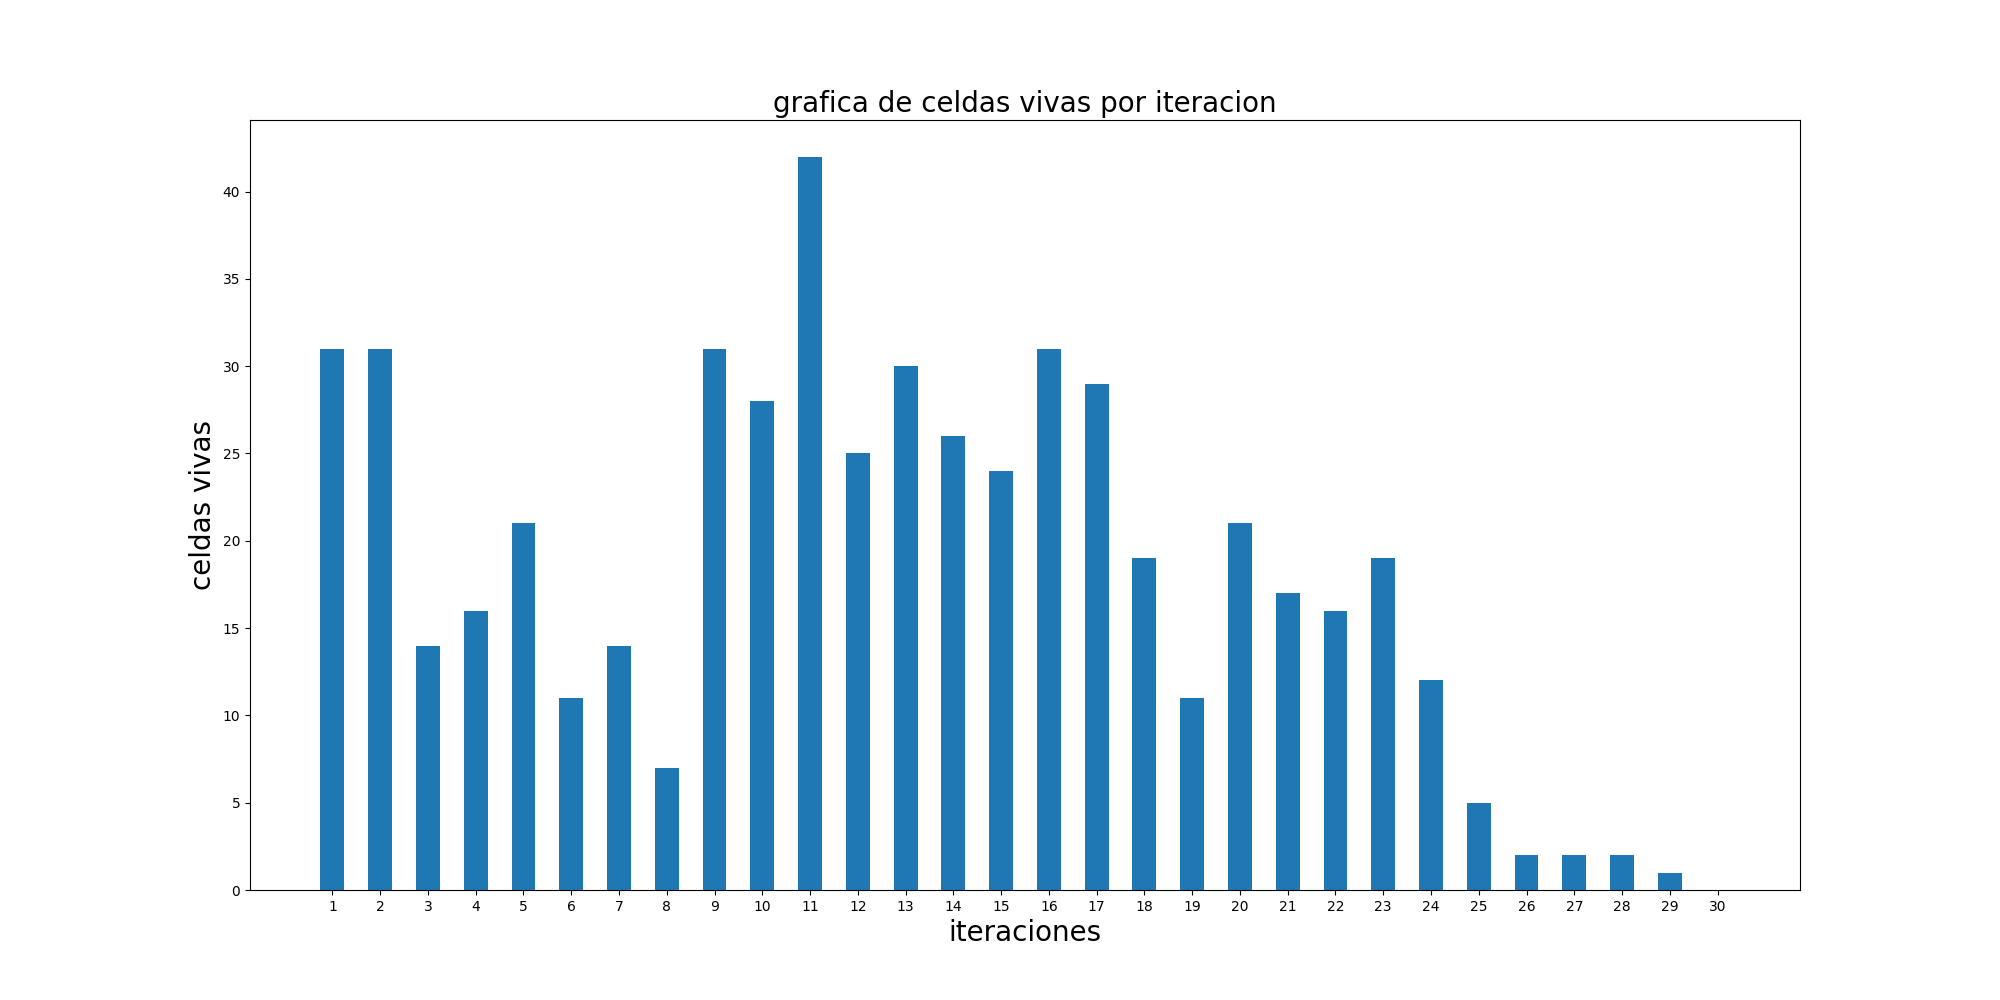
\includegraphics[scale=.4]{grafica_regla1.png}
  \label{regla1}
\end{figure}

La segunda regla aplicada se hacen dos condiciones, para el caso en que la celda central este viva y si tres vecinos exactamente estan vivos entonces se mantendra viva la celda pero si de lo contrario los vecinos no son igual a tres vivos entonces morira. Tambien se hizo condicion para crear vida en caso que la celda sea cero y si tres vecinos son vivos entonces esta celda vivira.
La figura \ref{regla2} muestra como en solo 4 iteraciones esta colonia desaparecio por completo ya que la condicion era muy dificil de que se diera, por eso dio saltos grandes al irse reduciendo de manera rapida.
\begin{verbatim}
        if pos == 1:  
            if L==3 : 
                matriz3[z]= 1
            else:
                matriz3[z]= 0
        if pos == 0:  
            if L == 3  :  
                matriz3[z]= 1
\end{verbatim}
\begin{figure}[H]
  \centering      
  \caption{grafica de resultados para la regla 2}  
  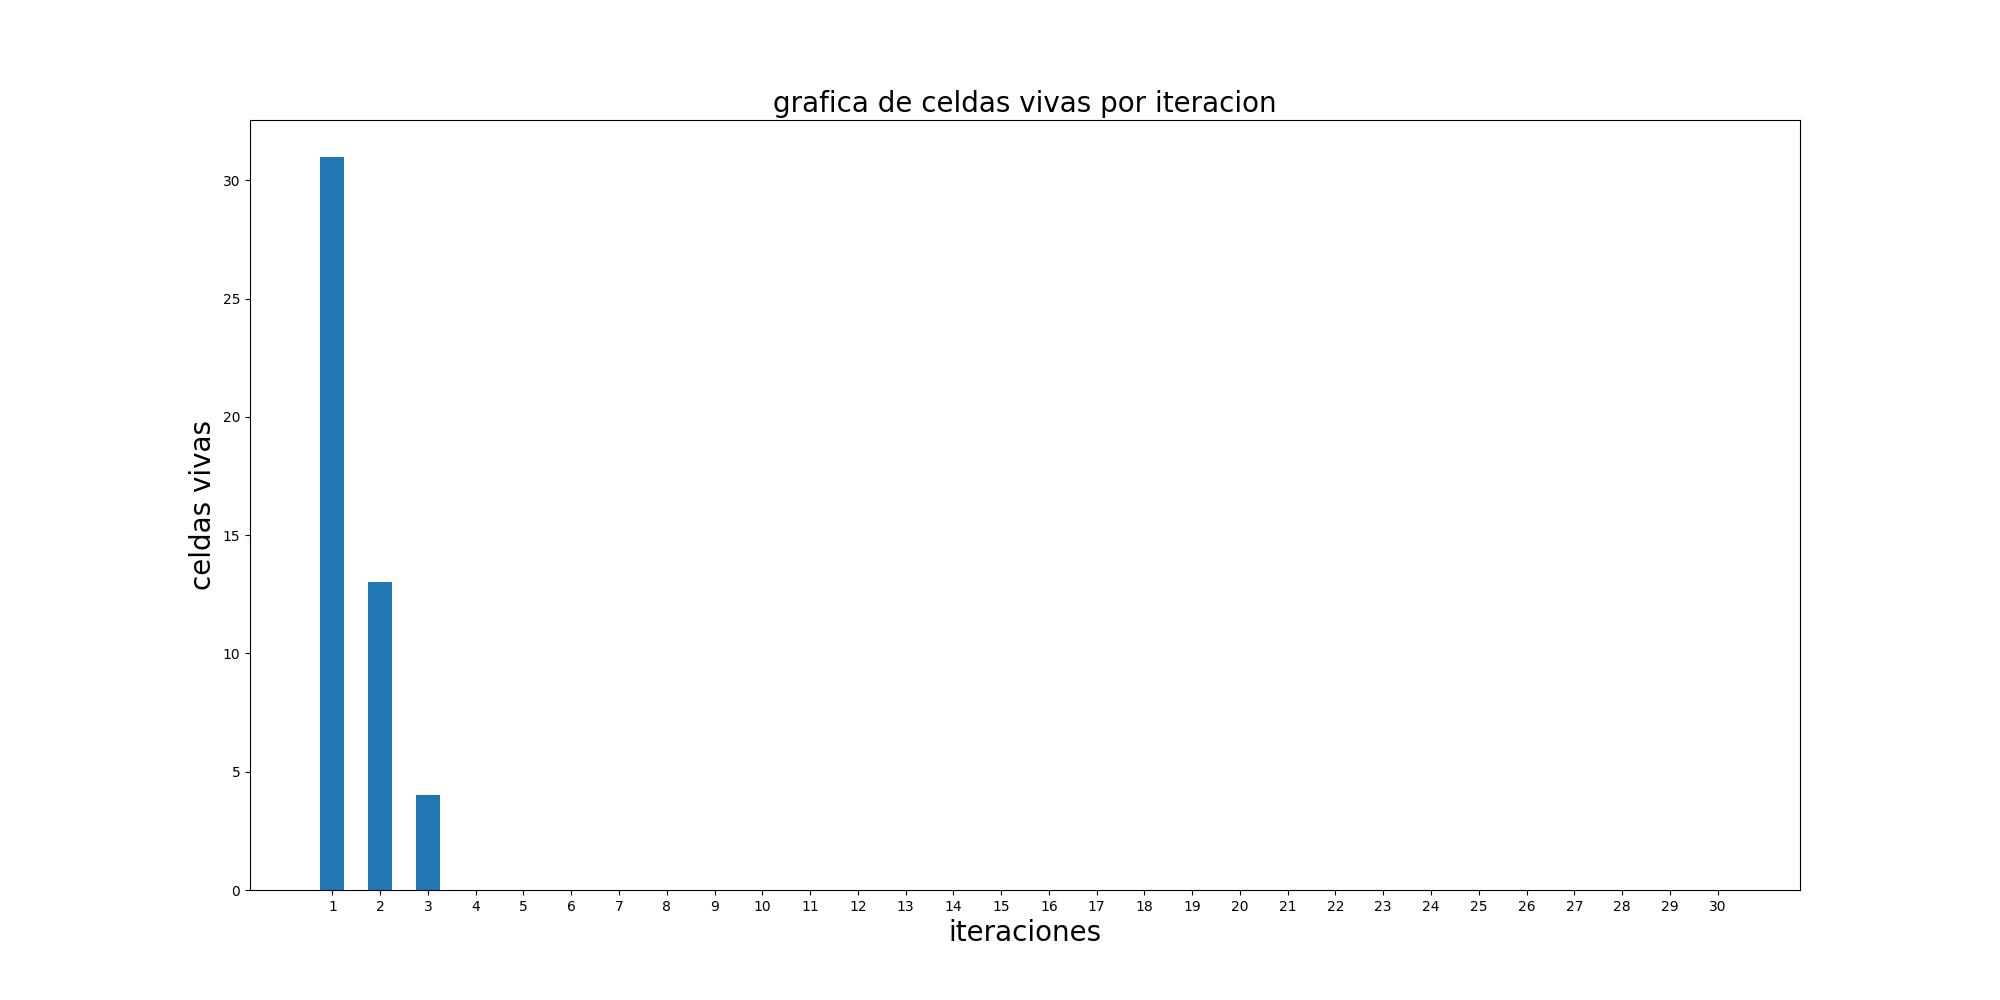
\includegraphics[scale=.4]{grafica_regla2.png}
  \label{regla2}
\end{figure}


La tercer regla consistio en una sola condicion de supervivencia en que si esta vivo el centro y si sus vecinos 4, 5, 6 estan vivos entonces este permanecera vivo y de lo contrario si no son estos morira la celda. Lo cual para literacion tres provoco que desapareciara toda la colonia de celdas figura \ref{regla3}.
\begin{verbatim}
        if pos == 1:  
            if 3< L <=6 : 
                matriz3[z]= 1           
            else:
                matriz[z]=0
\end{verbatim}
\begin{figure}[H]
  \centering      
  \caption{grafica de resultados para la regla 3}  
  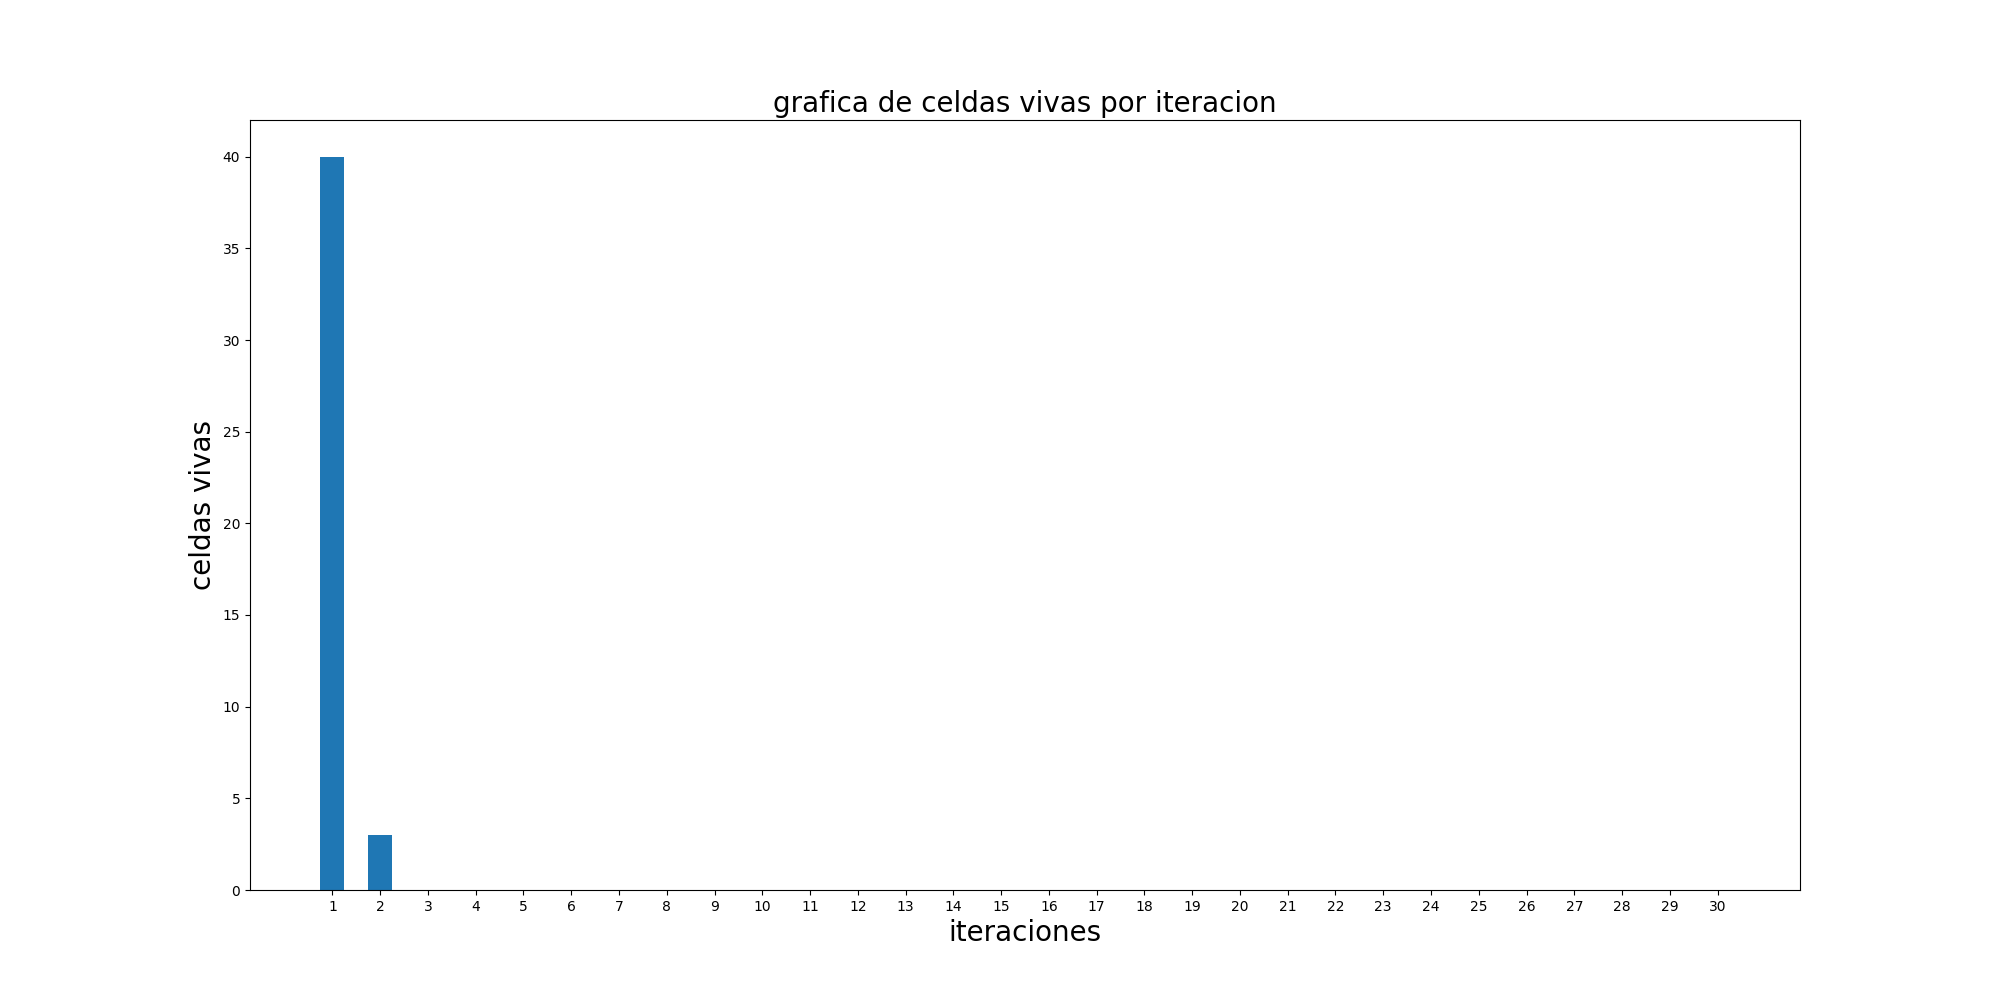
\includegraphics[scale=.4]{grafica_regla3.png}
  \label{regla3}
\end{figure}

La regla cuatro fue un caso diferente en su grafica de barras figura \ref{regla4} ya que se observo que no desaparecio a lo largo de 30 iteraciones sino de lo contrario aumento el numero de celdas vivas, esto como consecuencia de experimentar con las condiciones de supervivencia como lo muestra el codigo siguiente en que si la celda era uno y seis de sus vecinos vivian entonces este moria y caso contrario si la celda era cero y un vecino estaba vivo la celda cambia a uno, esta condicion fue la que deberia impedir que no murieran tantas celdas. 
\begin{verbatim}
      if pos == 1:  
            if L ==6 : 
                matriz3[z]= 0           
        if pos == 0:
            if L > 2
                 matriz3[z]= 1 
\end{verbatim}
\begin{figure}[H]
  \centering      
  \caption{grafica de resultados para la regla 4}  
  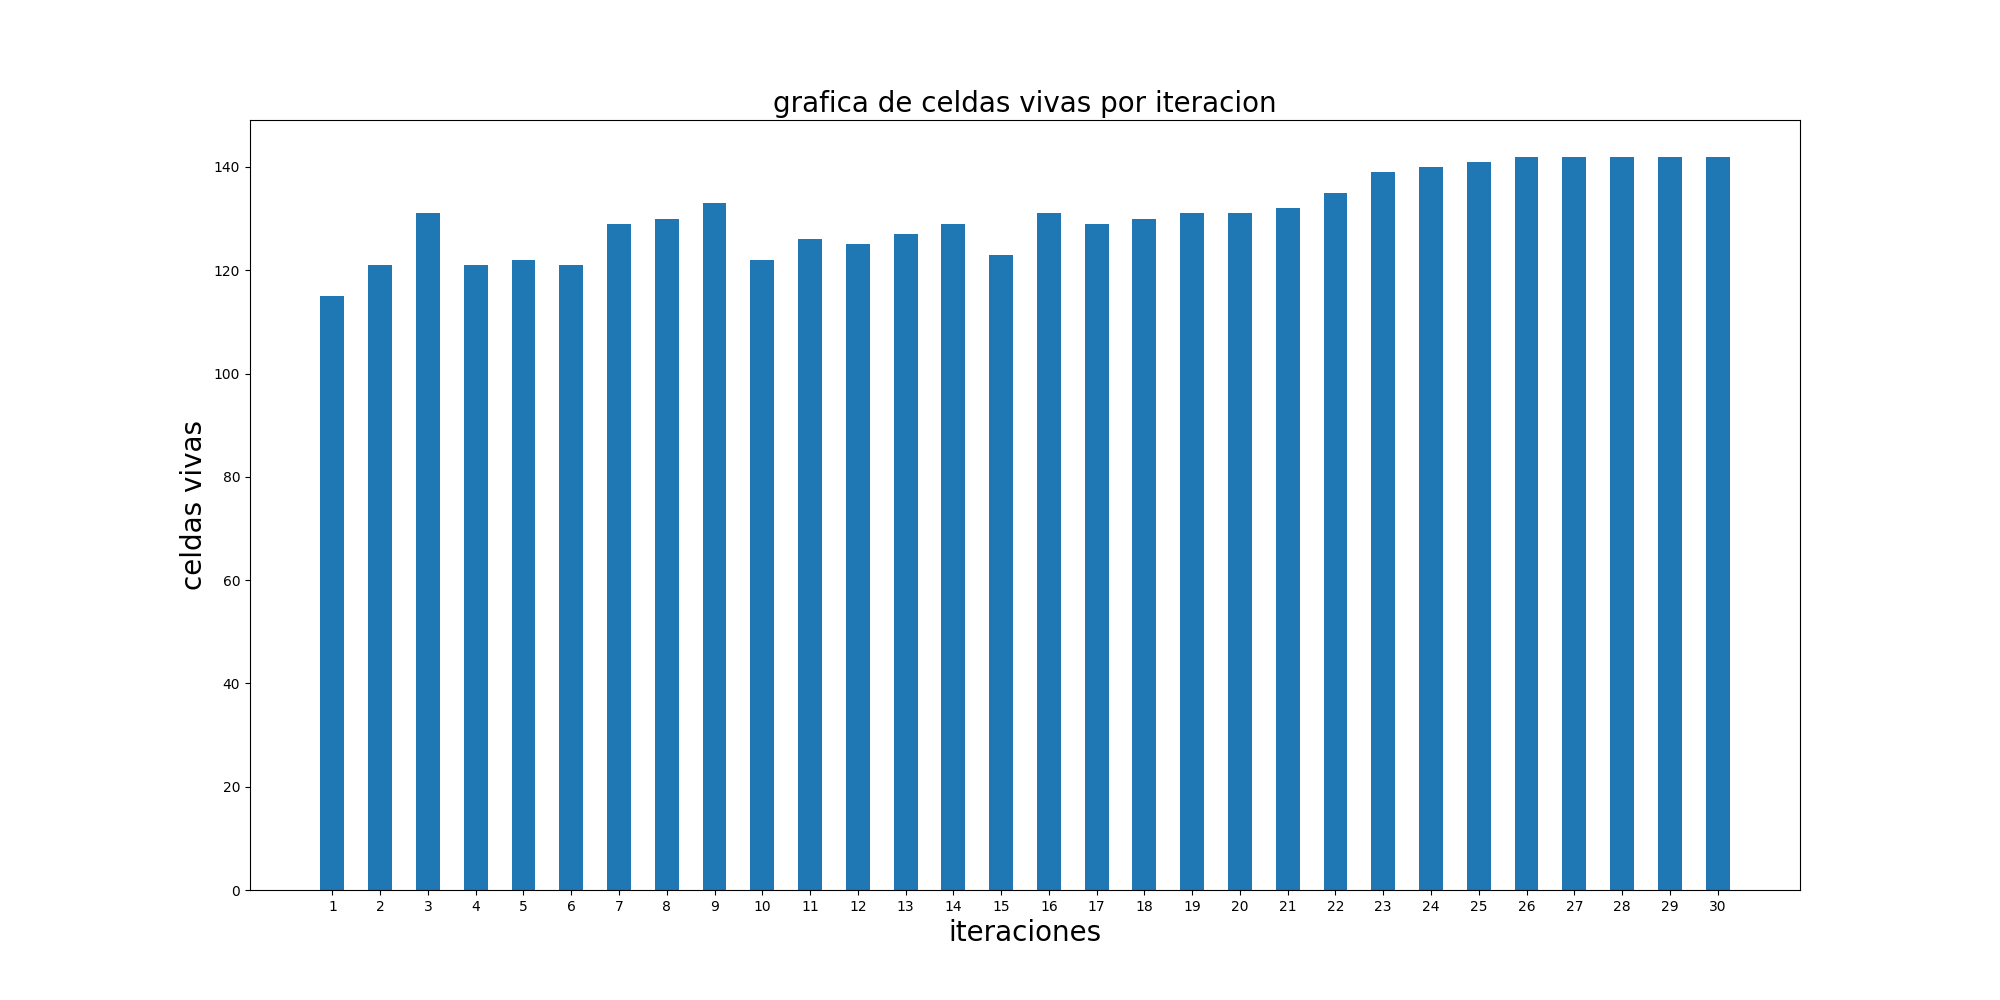
\includegraphics[scale=.4]{grafica_regla4.png}
  \label{regla4}
\end{figure}

Ya para la regla cinco se probo el caso en que la celda moriria solo si menos de tres vecinos estaban vivos y caso contrario unicamente si los vecinos cinco y seis estaban vivos. Los resultados se ven en la figura \ref{regla5} donde tuvo una duracion hasta la quinta iteracion para que desapareciera ya que la condicion de vida era muy dificil de coincidir.
\begin{verbatim}
        if pos == 1:  
            if L < 3 : 
                matriz3[z]= 0           
        if pos == 0:
            if 7 > L > 4
                 matriz3[z]= 1 
\end{verbatim}

\begin{figure}[H]
  \centering      
  \caption{grafica de resultados para la regla 5}  
  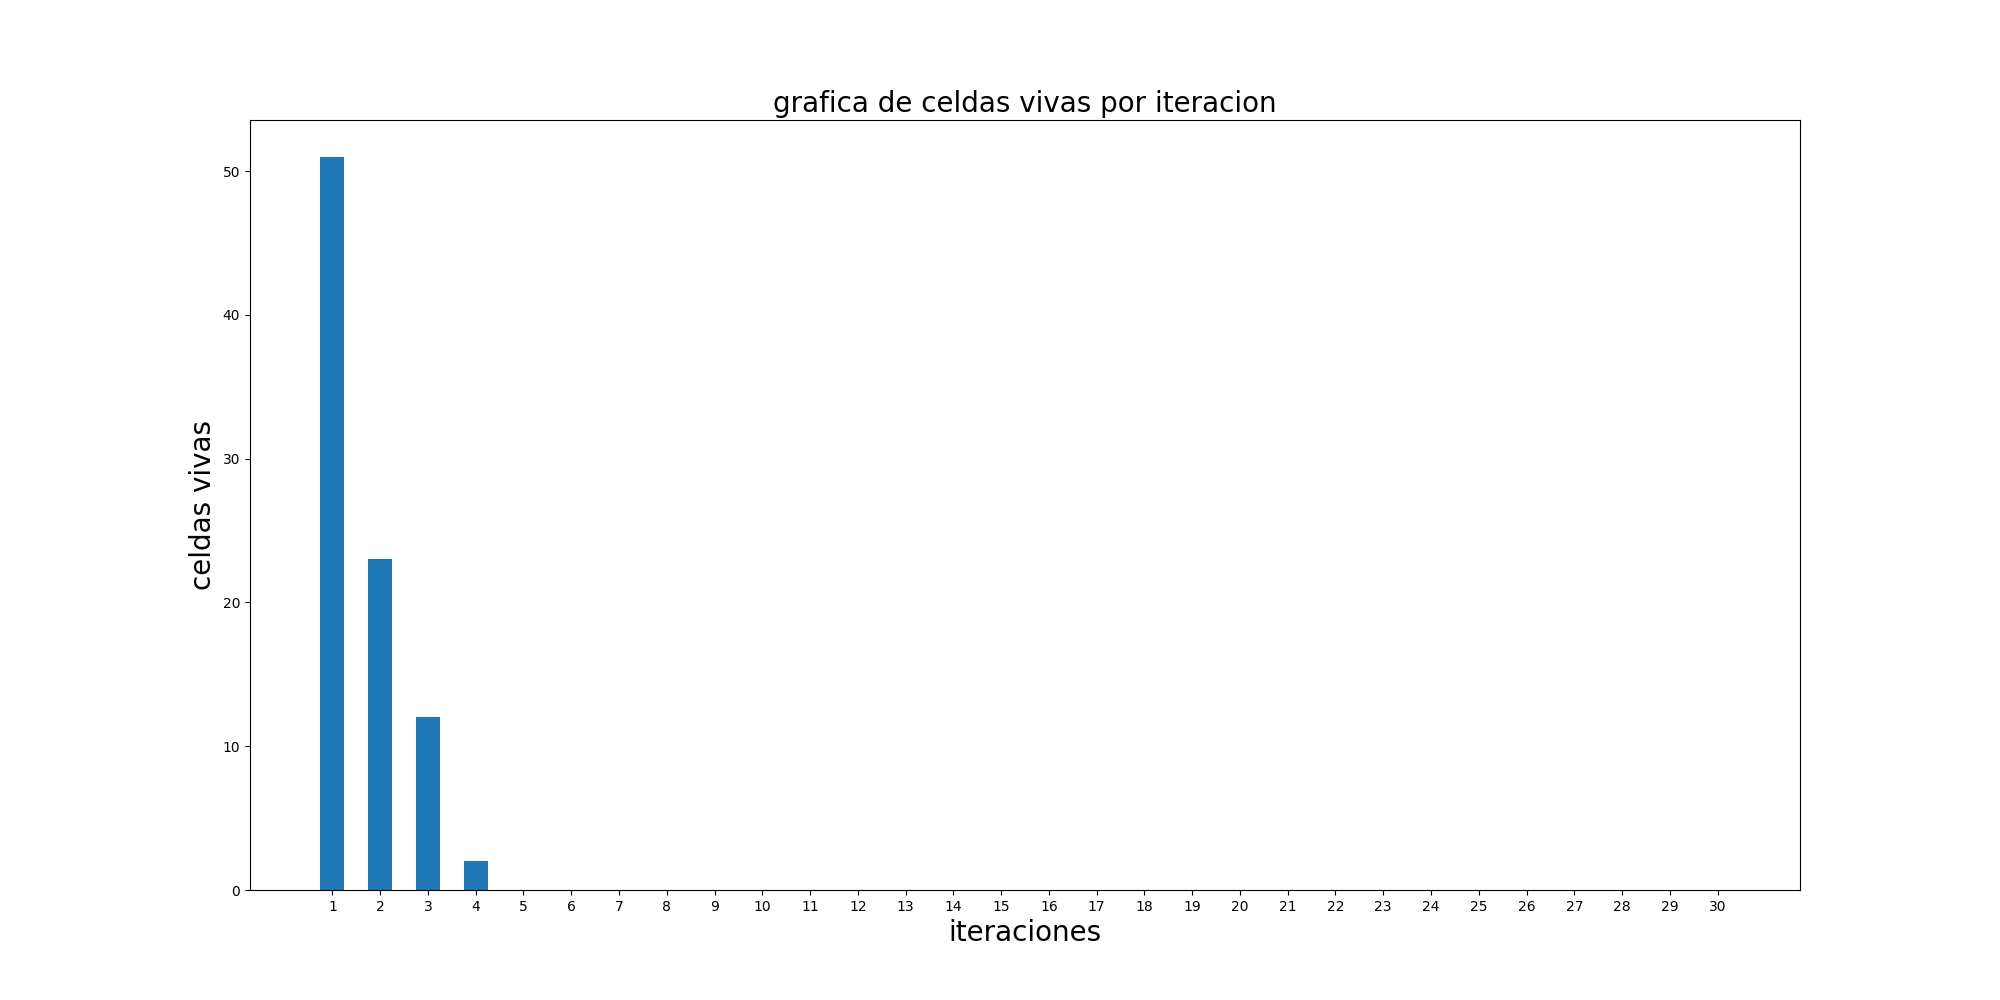
\includegraphics[scale=.4]{grafica_regla5.png}
  \label{regla5}
\end{figure}


\bibliography{referencias}
\bibliographystyle{plainnat}




\end{document}
